\subsection{Der photoelektrische Effekt}
\label{sec:photoelektrischer-effekt}

Die Entdeckung des Elektrons\index{Elektron} war eng mit elektrischen Entladungen,
Kathodenstrahlen\index{Kathodenstrahlen} und der Untersuchung geladener Teilchen verbunden.
Doch bald zeigte sich, dass Elektronen nicht nur in Entladungsröhren
auftreten. Sie können auch aus Metalloberflächen herausgelöst werden.

Ein besonders wichtiges Phänomen ist dabei der photoelektrische Effekt\index{Photoelektrischer Effekt}:
Trifft Licht geeigneter Frequenz\index{Frequenz} auf eine Metalloberfläche,
so können Elektronen aus dem Metall austreten.

Auf den ersten Blick scheint dies ein rein technischer Effekt zu sein.
Tatsächlich wurde er jedoch zu einem der entscheidenden Hinweise darauf,
dass Licht selbst eine quantenhafte Struktur besitzt.

\begin{HistoryBox}[Hertz und die erste Beobachtung]
	\label{box:hertz-photoeffekt}
	Heinrich Hertz\index{Hertz, Heinrich} beobachtete 1887 bei seinen Experimenten zu
	elektromagnetischen Wellen\index{Elektromagnetische Wellen}, dass ultraviolettes Licht
	elektrische Entladungen erleichtern kann. Damit war der photoelektrische Effekt
	noch nicht vollständig erklärt, aber experimentell sichtbar geworden.
\end{HistoryBox}

\subsubsection{Die Grundidee}

In einem Metall sind Elektronen nicht völlig frei.
Sie sind zwar beweglich und können zur elektrischen Leitfähigkeit beitragen,
aber sie befinden sich weiterhin im Einflussbereich des Metalls.

Damit ein Elektron die Metalloberfläche verlassen kann,
muss eine bestimmte Mindestenergie aufgebracht werden.
Diese Energie nennt man die Austrittsarbeit\index{Austrittsarbeit}.

\begin{PhysicsBox}[Austrittsarbeit]
	\label{box:austrittsarbeit}
	Die Austrittsarbeit ist die Mindestenergie, die ein Elektron benötigt,
	um eine Metalloberfläche verlassen zu können.
	Sie hängt vom Material der Oberfläche ab.
\end{PhysicsBox}

Fällt Licht auf die Oberfläche, so kann Energie auf Elektronen übertragen
werden. Ist diese Energie groß genug, verlassen Elektronen das Metall.
Diese austretenden Elektronen nennt man Photoelektronen\index{Photoelektronen}.

\begin{figure}[htbp]
	\centering
	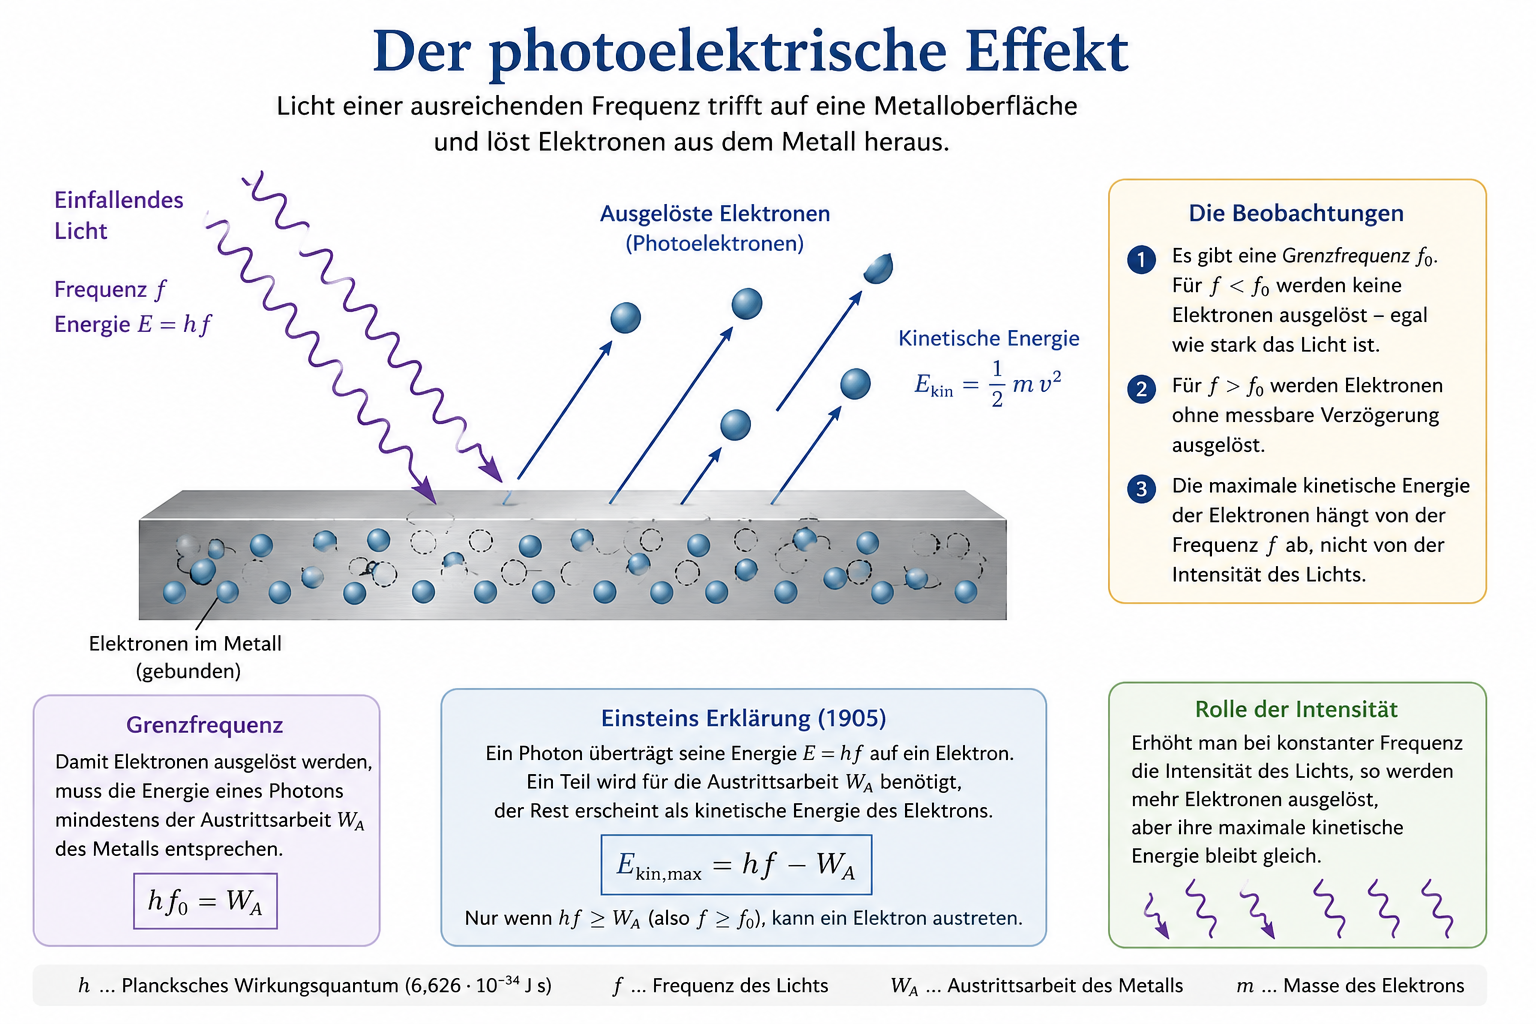
\includegraphics[width=\textwidth]{bilder/photoelektrischer_effekt.png}
	\caption{Schematische Darstellung des photoelektrischen Effekts: Licht ausreichender Frequenz trifft auf eine Metalloberfläche und löst Elektronen aus dem Metall heraus.}
	\label{fig:photoelektrischer-effekt}
\end{figure}

\subsubsection{Die klassische Erwartung}

Nach der klassischen Wellentheorie des Lichts\index{Wellentheorie des Lichts} hätte man erwartet,
dass die Energie des Lichts vor allem von seiner Intensität\index{Intensität} abhängt.
Je stärker das Licht, desto mehr Energie sollte auf die Elektronen
übertragen werden.

Daraus ergäben sich drei naheliegende Erwartungen:

\begin{itemize}
	\item Sehr intensives Licht sollte Elektronen auch dann herauslösen können,
	wenn seine Frequenz klein ist.
	\item Bei schwachem Licht sollte es eine gewisse Zeit dauern,
	bis ein Elektron genügend Energie aufgenommen hat.
	\item Die kinetische Energie\index{Kinetische Energie} der Elektronen sollte vor allem mit der
	Lichtintensität zunehmen.
\end{itemize}

Genau diese Erwartungen erfüllten sich jedoch nicht.

\begin{DidacticBox}[Die klassische Denkfalle]
	\label{box:klassische-denkfalle-photoeffekt}
	Klassisch würde man erwarten:
	Mehr Lichtintensität bedeutet mehr Energie pro Elektron.
	
	Experimentell zeigt sich aber:
	Die Energie der ausgelösten Elektronen hängt von der Frequenz des Lichts ab,
	nicht von seiner Intensität.
\end{DidacticBox}

\subsubsection{Die experimentellen Befunde}

Die Experimente zeigten ein klares und zunächst überraschendes Bild.

Erstens gibt es für jedes Material eine Grenzfrequenz\index{Grenzfrequenz}.
Unterhalb dieser Frequenz werden keine Elektronen ausgelöst,
ganz gleich, wie intensiv das Licht ist.

Zweitens erfolgt die Emission der Elektronen praktisch ohne messbare
Verzögerung. Das Elektron muss also nicht erst längere Zeit Energie
aus der Lichtwelle ansammeln.

Drittens bestimmt die Frequenz des Lichts die maximale kinetische Energie
der austretenden Elektronen. Die Intensität beeinflusst dagegen vor allem,
wie viele Elektronen austreten.

\begin{PhysicsBox}[Zentrale Beobachtung]
	\label{box:zentrale-beobachtung-photoeffekt}
	Beim photoelektrischen Effekt bestimmt die Frequenz des Lichts,
	ob Elektronen ausgelöst werden und welche maximale kinetische Energie
	sie besitzen. Die Intensität bestimmt vor allem die Anzahl der ausgelösten
	Elektronen.
\end{PhysicsBox}

Damit wurde klar:
Die klassische Wellentheorie konnte den Effekt nicht vollständig erklären.

\subsubsection{Einsteins Erklärung}

Albert Einstein\index{Einstein, Albert} schlug 1905 eine radikal neue Deutung vor.
Licht gibt seine Energie nicht beliebig kontinuierlich ab,
sondern in einzelnen Energiepaketen.

Diese Energiepakete werden heute Photonen\index{Photon} genannt.

Die Energie eines Photons ist proportional zur Frequenz des Lichts:

\[
E = h f
\]

Dabei ist \(h\) das Plancksche Wirkungsquantum\index{Plancksches Wirkungsquantum}
und \(f\) die Frequenz des Lichts.

Trifft ein Photon auf ein Elektron im Metall, so kann es seine Energie
auf dieses Elektron übertragen. Ein Teil dieser Energie wird benötigt,
um das Elektron aus dem Metall herauszulösen. Der verbleibende Teil
erscheint als kinetische Energie des Elektrons.

Damit ergibt sich:

\[
E_{\text{kin,max}} = h f - W_A
\]

Hierbei bezeichnet \(W_A\) die Austrittsarbeit des Metalls.

\begin{MathBox}[Einstein-Gleichung des Photoeffekts]
	\label{box:einstein-gleichung-photoeffekt}
	Für die maximale kinetische Energie der ausgelösten Elektronen gilt:
	
	\[
	E_{\text{kin,max}} = h f - W_A
	\]
	
	Nur wenn
	
	\[
	h f \geq W_A
	\]
	
	ist, können Elektronen aus dem Metall austreten.
\end{MathBox}

Diese Gleichung erklärt sofort die experimentellen Befunde.

Ist die Frequenz zu klein, besitzt jedes einzelne Photon zu wenig Energie.
Dann können keine Elektronen austreten, auch wenn sehr viele Photonen
auf die Oberfläche treffen.

Erhöht man dagegen die Intensität bei ausreichender Frequenz,
treffen mehr Photonen auf die Oberfläche.
Dann werden mehr Elektronen ausgelöst, aber ihre maximale Energie
ändert sich nicht wesentlich.

\subsubsection{Bedeutung für das Elektron}

Für die Geschichte des Elektrons ist der photoelektrische Effekt
aus mehreren Gründen wichtig.

Er zeigt erstens, dass Elektronen reale, aus Materie herauslösbare
geladene Teilchen sind. Sie befinden sich nicht nur in Kathodenstrahlen,
sondern sind Bestandteil gewöhnlicher Materie.

Zweitens erlaubt der Effekt eine genaue Untersuchung der Energie von
Elektronen. Über Gegenspannungsmethoden\index{Gegenspannungsmethode} kann man messen,
welche maximale kinetische Energie die Photoelektronen besitzen.

Drittens verbindet der photoelektrische Effekt die Elektronentheorie
mit der Lichtquantenhypothese\index{Lichtquantenhypothese}. Das Elektron wird hier zum direkten
Nachweisteilchen für die quantenhafte Energieübertragung des Lichts.

\begin{DidacticBox}[Warum der Effekt so wichtig ist]
	\label{box:bedeutung-photoeffekt-elektron}
	Der photoelektrische Effekt zeigt zwei Dinge zugleich:
	Elektronen sind reale Teilchen in der Materie,
	und Licht überträgt Energie in einzelnen Quanten.
	Damit verbindet der Effekt Elektronentheorie und Quantentheorie.
\end{DidacticBox}

\subsubsection{Übergang zur Quantenphysik}

Der photoelektrische Effekt markiert einen Wendepunkt.
Er zeigte, dass die klassische Vorstellung von Licht als rein
kontinuierlicher Welle nicht ausreicht.

Gleichzeitig wurde deutlich:
Auch das Elektron kann nicht mehr nur als klassisches kleines Teilchen
verstanden werden. Seine Wechselwirkung mit Licht führt direkt in die
Quantenphysik\index{Quantenphysik}.

Im weiteren Verlauf der Physikgeschichte wurde daraus ein neues Bild
der Materie entwickelt. Elektronen sind Bestandteile der Atome,
tragen elektrische Ladung, besitzen Masse und zeigen in geeigneten
Experimenten auch Welleneigenschaften\index{Welleneigenschaften}.

Der photoelektrische Effekt steht damit an einer Schlüsselstelle:
Er beginnt bei einer Metalloberfläche und führt mitten hinein in die
moderne Quantenmechanik\index{Quantenmechanik}.

\begin{HistoryBox}[Einsteins Nobelpreis]
	\label{box:einstein-nobelpreis-photoeffekt}
	Albert Einstein erhielt den Nobelpreis für Physik\index{Nobelpreis für Physik} des Jahres 1921
	nicht für die Relativitätstheorie\index{Relativitätstheorie}, sondern insbesondere für seine
	Erklärung des photoelektrischen Effekts. Das zeigt, welche zentrale
	Bedeutung dieser Effekt für die Entstehung der Quantentheorie hatte.
\end{HistoryBox}

\begin{NoteBox}[Einordnung im roten Faden]
	\label{box:einordnung-photoeffekt}
	Für dieses Buch ist der photoelektrische Effekt eine Brücke:
	Er verbindet die Entdeckung des Elektrons mit der späteren Quantentheorie
	und zeigt, warum das Elektron nicht nur ein klassisches Teilchen,
	sondern ein fundamentales Quantenobjekt ist.
\end{NoteBox}